\chapter{Docker} \label{ch:docker}

Negli ultimi anni numerose aziende che forniscono servizi agli utenti si sono trovate in serie difficoltà a causa dell' aumento sempre costante del numero
dei propri utenti e delle richieste di questi ultimi. Tali aziende si sono trovate quindi nella posizione di dover incrementare proporzionalmente le loro risorse disponibili, sia hardware che software, e di dover
assumere sempre più frequentemente del personale altamente specializzato per gestirle. Questa situazione di crisi ha portato ad un cambio di prospettiva in ambito aziendale, orientando l'attenzione verso un sistema di virtualizzazione
basato sull'utilizzo dei container invece che con le classiche macchine virtuali. Così facendo si è trovata una valida soluzione a questo problema, in quanto grazie alle loro caratteristiche i container consentono di garantire
la qualità del servizio offerto dalle aziende, ottimizzando l'utilizzo delle risorse hardware già in uso, senza la necessità di effettuare ulteriori investimenti significativi in hardware o personale aggiuntivo.\\
L'obiettivo di questo capitolo è di fornire una descrizione approfondita di una delle tecnologie più diffuse ed utilizzate in questo ambito, Docker\cite{docker-docs}. Inoltre viene anche descritto l'utilizzo di uno strumento, docker-compose, molto utile per 
creare e gestire applicazioni multi-container. Nella parte finale del capitolo è infine possibile trovare una descrizione e degli esempi su come eseguire il networking all'interno dei container.

\section{Differenze fra Container e Macchine Virtuali} 

Prima di scendere nello specifico descrivendo il funzionamento di docker all'interno di un sistema operativo è necessario definire nel dettaglio cosa sia una macchina virtuale e cosa un container e perchè è più efficiente la seconda soluzione rispetto alla prima.\\
Per quanto riguarda le macchine virtuali una definizione ci viene fornita dal sito ufficiale di VMware \cite{vmware}:\\
"Una Macchina Virtuale (VM) è una risorsa di elaborazione che utilizza software al posto di un computer fisico per eseguire programmi e distribuire applicazioni. Una o più macchine virtuali (guest) vengono eseguite su una macchina fisica (host). 
Ogni macchina virtuale esegue il proprio sistema operativo e funziona in modo separato dalle altre VM, anche quando sono tutte in esecuzione sulla stessa macchina host. Ciò significa che, ad esempio, una macchina virtuale con sistema operativo MacOS può essere eseguita su un PC fisico."\\

Sotto la prospettiva dei container, è possibile ottenere una definizione precisa consultando la documentazione ufficiale di Docker\cite{docker-container}.\\
"Un container è  un'unità standard di software che raggruppa il codice e tutte le sue dipendenze in modo che l'applicazione possa essere eseguita rapidamente e in modo affidabile da un ambiente di calcolo all'altro."\\

Seppur le due definizioni possano sembrare molto simili, la struttura software che sta dietro ad entrambe le tecniche di virtualizzazione è diversa, come viene mostrato nella seguente figura:\\


\begin{figure}[h]  % 'h' significa che la figura viene posizionata qui
    \centering
    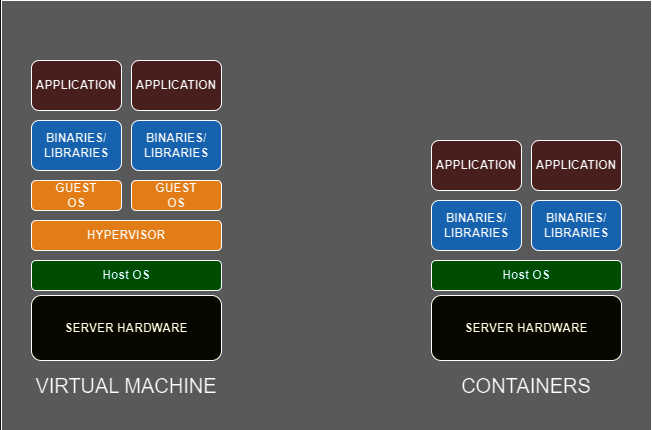
\includegraphics[width=1\textwidth]{VMvsContainers.png}  % Sostituisci 'nome_immagine' con il nome del tuo file immagine e l'estensione
    \caption{Architettura Virtual Machine e Containers}
    \label{fig:VMvsContainers}
\end{figure}
 
Le macchine virtuali hanno infatti una struttura più complessa rispetto ai container. È infatti presente un hypervisor\cite{hypervisor}, che è un software che permette di creare e gestire le macchine virtuali in maniera veloce, efficiente, flessibile e portabile.
Sopra all'hypervisor ogni macchina virtuale ha il suo proprio sistema operativo, costringendo l'host OS ad allocare numerose risorse per istanziare anche solo 1 macchina virtuale. Si può notare come questa soluzione sia difficlmente scalabile perchè
ciò porta il server hardware sul quale poggia tutto il sistema ad essere ulteriormente stressato con l'aggiunta di ogni macchina virtuale. Viceversa, i container richiedono solo le risorse minime necessaria a fare funzionare l'applicazione di turno, installando solo i file binari e le librerie necessarie.\\
Più in generale le caratteristiche vantaggiose dei container rispetto alle macchine virtuali sono riassunte dalle seguenti parole chiave:\\


\begin{itemize}
    \item \textbf{Modularità}: avere la possibilità di creare un container per ogni possibile task permette di suddividere i container in vari moduli, ognuno che svolge una sepcifica funzione del progetto di riferimento. Operando in tale direzione, è possibile sviluppare progetti con un approccio Bottom-Up
        , portando ad un ambiente di testing e validation più veloce ed immediato sui singoli moduli.
    \item \textbf{Isolamento}: ogni container che esegue una immagine viene visto come un ambiente isolato, indipendente dagli altri container in esecuzione. Questo approccio semplifica notevolmente l'individuazione di possibili bug ed errori nel progetto.
    \item \textbf{Peso in Memoria}: come analizzato nel lavoro di Martin Lindström\cite{performance-container}, differentemente dalle macchine virtuali, i container sono delle virtualizzazioni molto più leggere e che richiedono meno risorse alla macchina ospitante. Questo è derivato dal fatto che i container contengono solo lo stretto necessario all'applicazione per funzionare correttamente,
        mentre le VM hanno bisogno anche di istanziare un proprio sistema operativo, che richiede una discreta quantità di spazio.
    \item \textbf{Scalabilità}: Avendo un peso molto ridotto rispetto alle macchine virtuali, la necessità di aumentare le performance e le dimensioni di un progetto trova nei container un ottimo fattore di scalabilità. È  infatti possibile scalare i sistemi sia verticalmente, perchè all'aumentare delle risorse del sistema operativo ospitante corrisponde un aumento della velocità di reazione dei container
    che orizzontalmente, perchè aggiungere una feature corrisponde nell'aggiungere un container al sistema già funzionante. 
    \item \textbf{Condivisone Risorse}: Attraverso i file di configurazione dei container è possibile condividere file con il container, che nell'ambiente isolato verranno considerate come risorse dedicate, anche se in realtà sono condivise. Ciò estende questa funzionalità se si mettono in comune le stesse risorse per più container. In questo caso sulle risorse verrà messo un lock che bloccherà le risorse fino a che
        uno dei container non abbia finito di utilizzarle, rilasciandole.
    \item \textbf{Fast Boot}:Non dovendo dipendere da nessun sistema operativo, i container possono avviarsi ed essere operativi molto più velocemente rispetto alle macchine virtuali.
    \item \textbf{Operazioni su disco}: Avendo un collegamento diretto con il sistema operativo le operazioni su  disco (scrittura, lettura e cancellazione) sono più veloci, portando ad un aumento delle performance per processi parallelizzabili.
\end{itemize}

\newpage

\section{Docker e la sua architettura}

Tra le piattaforme software disponibili per istanziare e gestire containers per applicazioni Docker riveste il ruolo di software leader nel settore.
Nato nel 2013 e progettato da Solomon Hykes nell'azienda dotCloud, Docker è un progetto open source. La differenza fondamentale dagli altri software è che
basa la maggior parte delle operazioni eseguibili su un demone chiamato appunto Docker, che svolge le operazioni di istanziazione dei container e la loro gestione.
Al fine di garantire ciò, il demone richiede come file di input delle \textit{"Immagini"}. Come è descritto nella documentazione di Docker\cite{docker-container}: 
"Un'immagine di container Docker è un pacchetto leggero, autonomo ed eseguibile di software che include tutto il necessario per eseguire un'applicazione: codice, runtime, strumenti di sistema, librerie di sistema e impostazioni."\\

L'architettura di Docker sfrutta il meccanismo client-server, della quale viene mostrata una rappresentazione:\\

\begin{figure}[h]  % 'h' significa che la figura viene posizionata qui
    \centering
    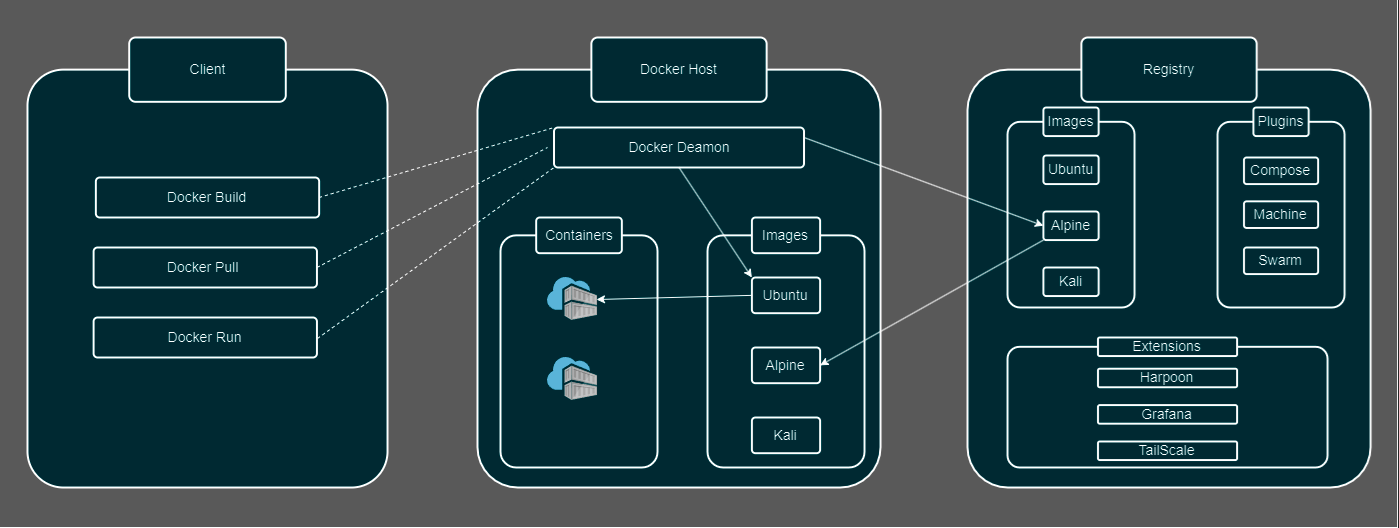
\includegraphics[width=1\textwidth]{Docker_Architecture.png}  % Sostituisci 'nome_immagine' con il nome del tuo file immagine e l'estensione
    \caption{Architettura Docker}
    \label{fig:DockerArchitecture}
\end{figure}

Di seguito una spiegazione di tutti gli elementi che intervengono nella creazione di un container:

\begin{itemize}
    \item \textbf{Docker Client}: Rappresenta la macchina fisica nel quale è installato Docker. Può comunicare con il controller principale (Docker Host) tramite delle Rest API.
    Le chiamate che il client può effettuare sono le seguenti:
        \begin{itemize}
            \item \textit{Docker Pull}: viene utilizzato per scaricare un'immagine da un Registro. Il demone controllerà se questa immagine è presente nel registro locale indicato, altrimenti andrà a cercare online
                la versione più recente dal registro predefinito di Docker Hub.
            \item \textit{Docker Build}: questo comando permette la creazione di un'immagine dato un file di configurazione definito dall utente (deve avere il nome di Dockerfile) e una cartella di riferimento.
            \item \textit{Docker Run}: questa chiamata fa creare al demone un container con l'immagine specificata da linea di comando ed avvia il container.
        \end{itemize}
    \item \textbf{Docker Deamon}: è il cuore dell'architettura di Docker. Il ruolo del docker deamon(anche chiamato dockerd) è di ascoltare le richieste tramite call API del client e gestire il registro Docker dove sono contenute
        le immagini, i plugin e le estensioni. Inoltre può comunicare con altri demoni per gestire i servizi Docker.
    \item \textbf{Docker Registry}: è  una zona di memoria che memorizza le immagini Docker. In questa zona sono anche presenti eventuali plugin installati su Docker e le estensioni sviluppate per sfruttare i servizi di Docker.
        Talvolta potrebbe capitare che le immagini ricercate nel registro non sono presenti, ed in questo caso viene effettuato un collegamento diretto con un registro pubblico online definito Docker Hub per poter usufruire di alcune
        immagini già pronte.
\end{itemize}


Ha senso inserire anche come si scrive un dockerfile con esempi di comando o no?

\section{Il tool Compose}
Come si è potuto notare nella sezione precedente, Docker garantisce un grado di flessibilità molto elevato che consente di creare sia container che svolgono ruoli molto semplici che container più articolati che richiedono anche l'installazione di diverse
librerie tramite Dockerfile. Tuttavia può capitare molto spesso che l'ambiente isolato di un container all'altro sia una limitazione in quanto per svolgere determinati task due o più macchine virtuali devono potere comunicare efficacemente, inoltre la gestione
di reti complesse tramite singoli Dockerfile e linea di comando può risultare tediosa e molto scomoda da utilizzare. Basti pensare che nel caso di un container non funzionante bisognerebbe modificare non solo il Dockerfile del singolo elemento, ma anche rieseguire tutte le chiamate
di sistema per fare rebuild dell'ambiente virtuale. \\
Per venire incontro a questi problemi molto comuni nello sviluppo di applicazioni aziendali, Docker propone delle soluzioni innovative e che cercano non solo di risolvere i problemi sopracitati , ma anche di introdurre dei meccanismi di semplificazione per la gestione di reti complesse.




\section{Networking}